\documentclass[11pt,a4paper]{report}
\usepackage[textwidth=37em,vmargin=30mm]{geometry}
\usepackage{calc,xunicode,amsmath,amssymb,paralist,enumitem,tabu,booktabs,datetime2,xeCJK,xeCJKfntef,listings}
\usepackage{tocloft,fancyhdr,tcolorbox,xcolor,graphicx,eso-pic,xltxtra,xelatexemoji}

\newcommand{\envyear}[0]{2024}
\newcommand{\envdatestr}[0]{2024-10-25}
\newcommand{\envfinaldir}[0]{webdb/2024/20241025/final}

\usepackage[hidelinks]{hyperref}
\hypersetup{
    colorlinks=false,
    pdfpagemode=FullScreen,
    pdftitle={Web Digest - \envdatestr}
}

\setlength{\cftbeforechapskip}{10pt}
\renewcommand{\cftchapfont}{\rmfamily\bfseries\large\raggedright}
\setlength{\cftbeforesecskip}{2pt}
\renewcommand{\cftsecfont}{\sffamily\small\raggedright}

\setdefaultleftmargin{2em}{2em}{1em}{1em}{1em}{1em}

\usepackage{xeCJK,xeCJKfntef}
\xeCJKsetup{PunctStyle=plain,RubberPunctSkip=false,CJKglue=\strut\hskip 0pt plus 0.1em minus 0.05em,CJKecglue=\strut\hskip 0.22em plus 0.2em}
\XeTeXlinebreaklocale "zh"
\XeTeXlinebreakskip = 0pt


\setmainfont{Brygada 1918}
\setromanfont{Brygada 1918}
\setsansfont{IBM Plex Sans}
\setmonofont{JetBrains Mono NL}
\setCJKmainfont{Noto Serif CJK SC}
\setCJKromanfont{Noto Serif CJK SC}
\setCJKsansfont{Noto Sans CJK SC}
\setCJKmonofont{Noto Sans CJK SC}

\setlength{\parindent}{0pt}
\setlength{\parskip}{8pt}
\linespread{1.15}

\lstset{
	basicstyle=\ttfamily\footnotesize,
	numbersep=5pt,
	backgroundcolor=\color{black!5},
	showspaces=false,
	showstringspaces=false,
	showtabs=false,
	tabsize=2,
	captionpos=b,
	breaklines=true,
	breakatwhitespace=true,
	breakautoindent=true,
	linewidth=\textwidth
}






\newcommand{\coverpic}[2]{
    % argv: itemurl, authorname
    Cover photo by #2~~(\href{#1}{#1})
}
\newcommand{\makeheader}[0]{
    \begin{titlepage}
        % \newgeometry{hmargin=15mm,tmargin=21mm,bmargin=12mm}
        \begin{center}
            
            \rmfamily\scshape
            \fontspec{BaskervilleF}
            \fontspec{Old Standard}
            \fontsize{59pt}{70pt}\selectfont
            WEB\hfill DIGEST
            
            \vfill
            % \vskip 30pt
            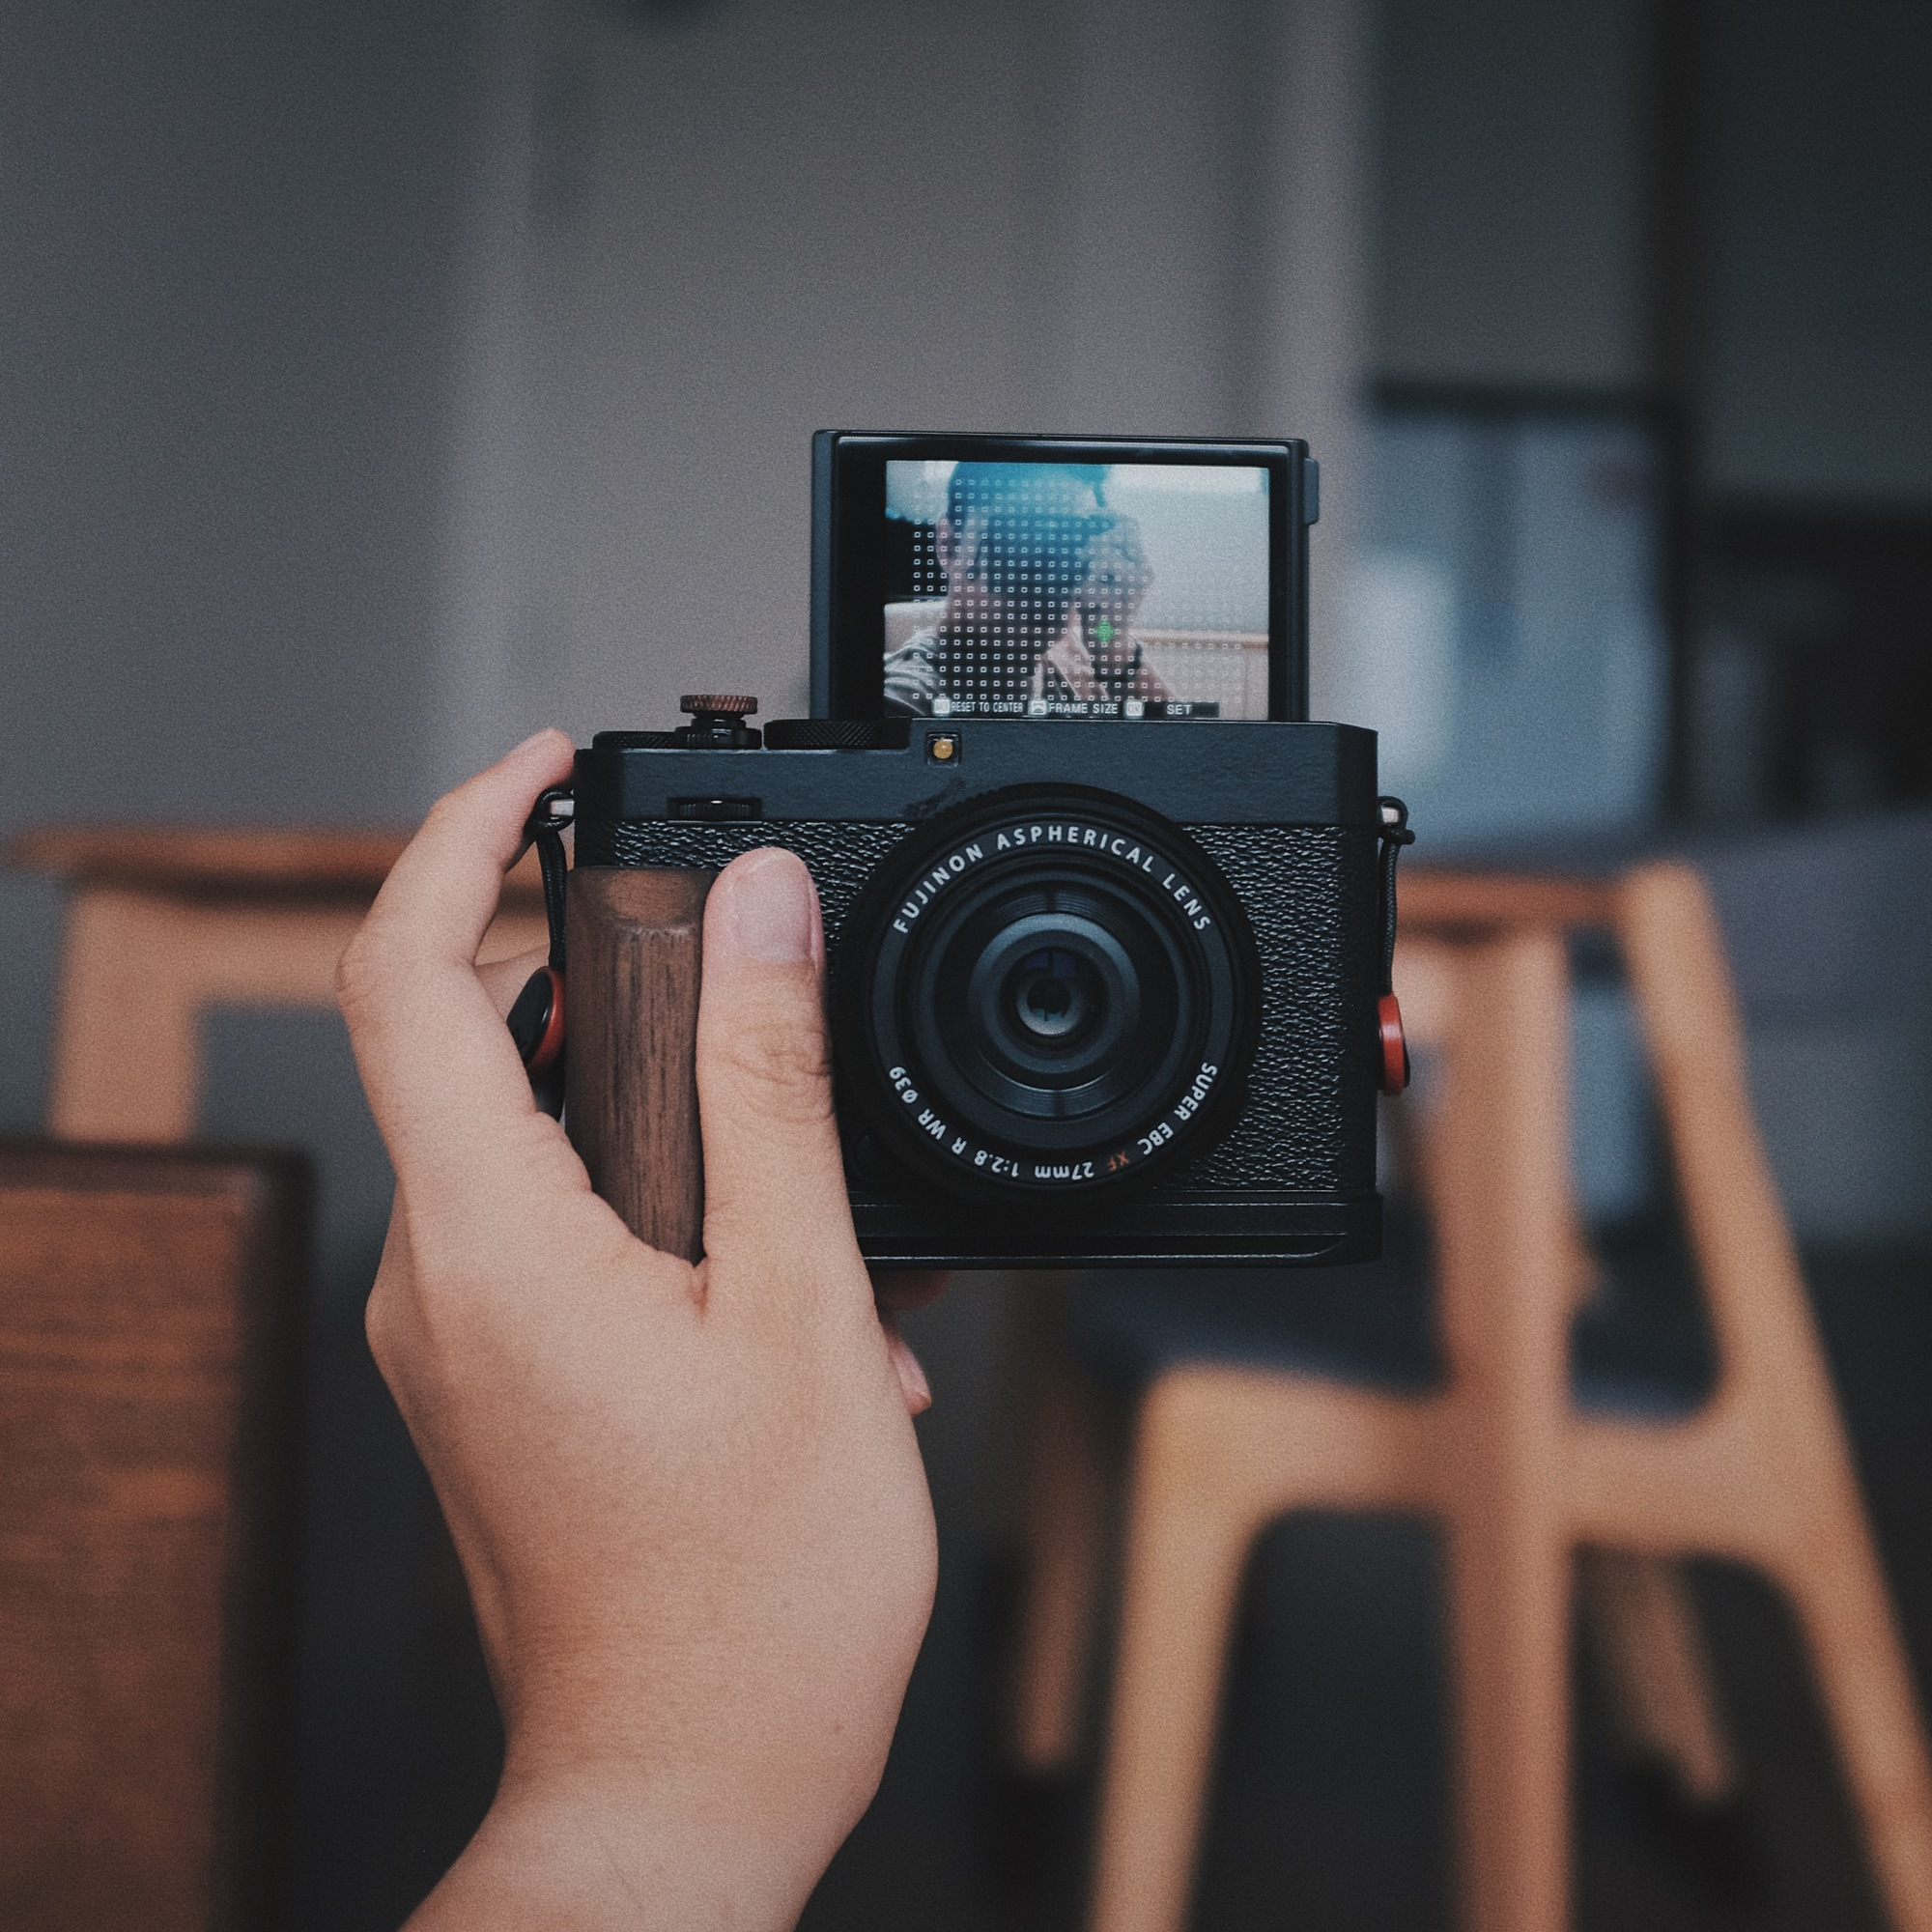
\includegraphics[width=\linewidth]{\envfinaldir/coverpic-prod.jpg}\par
            % \vskip 30pt
            \vfill

            \normalsize\rmfamily\scshape
            \copyright{} The Web Digest Project \hfill\large \envdatestr
        \end{center}
    \end{titlepage}
    % \restoregeometry
}
\newcommand{\simplehref}[1]{%
    \textcolor{blue!80!green}{\href{#1}{#1}}%
}
\renewcommand{\contentsname}{\center\Huge\sffamily\bfseries Contents\par\vskip 20pt}
\newcounter{ipartcounter}
\setcounter{ipartcounter}{0}
\newcommand{\ipart}[1]{
    % \vskip 20pt
    \clearpage
    \stepcounter{ipartcounter}
    \phantomsection
    \addcontentsline{toc}{chapter}{#1}
    % \begin{center}
    %     \Huge
    %     \sffamily\bfseries
    %     #1
    % \end{center}
    % \vskip 20pt plus 7pt
}
\newcounter{ichaptercounter}
\setcounter{ichaptercounter}{0}
\newcommand{\ichapter}[1]{
    % \vskip 20pt
    \clearpage
    \stepcounter{ichaptercounter}
    \phantomsection
    \addcontentsline{toc}{section}{\numberline{\arabic{ichaptercounter}}#1}
    \begin{center}
        \Huge
        \sffamily\bfseries
        #1
    \end{center}
    \vskip 20pt plus 7pt
}
\newcommand{\entrytitlefont}[1]{\subsection*{\raggedright\Large\sffamily\bfseries#1}}
\newcommand{\entryitemGeneric}[2]{
    % argv: title, url
    \parbox{\linewidth}{
        \entrytitlefont{#1}\par\vskip 5pt
        \footnotesize\ttfamily\mdseries
        \simplehref{#2}
    }\vskip 11pt plus 11pt minus 1pt
}
\newcommand{\entryitemGithub}[3]{
    % argv: title, url, desc
    \parbox{\linewidth}{
        \entrytitlefont{#1}\par\vskip 5pt
        \footnotesize\ttfamily\mdseries
        \simplehref{#2}\par\vskip 5pt
        \small\rmfamily\mdseries#3
    }\vskip 11pt plus 11pt minus 1pt
}
\newcommand{\entryitemAp}[3]{
    % argv: title, url, desc
    \parbox{\linewidth}{
        \entrytitlefont{#1}\par\vskip 5pt
        \footnotesize\ttfamily\mdseries
        \simplehref{#2}\par\vskip 5pt
        \small\rmfamily\mdseries#3
    }\vskip 11pt plus 11pt minus 1pt
}
\newcommand{\entryitemHackernews}[3]{
    % argv: title, hnurl, rawurl
    % \parbox{\linewidth}{
    %     \entrytitlefont{#1}\par\vskip 5pt
    %     \footnotesize\ttfamily\mdseries
    %     \simplehref{#3}\par
    %     \textcolor{black!50}{\href{#2}{#2}}
    % }\vskip 11pt plus 11pt minus 1pt
    \begin{minipage}{\linewidth}
            \entrytitlefont{#1}\par\vskip 5pt
            \footnotesize\ttfamily\mdseries
            \simplehref{#3}\par
            \textcolor{black!50}{\href{#2}{#2}}
    \end{minipage}\par\vskip 11pt plus 11pt minus 1pt
}







\begin{document}

\makeheader

\tableofcontents\clearpage




\ipart{Developers}
\ichapter{Hacker News}
\entryitemTwoLinks{Quantized Llama models with increased speed and a reduced memory footprint}{https://news.ycombinator.com/item?id=41938473}{https://ai.meta.com/blog/meta-llama-quantized-lightweight-models/?\_fb\_noscript=1}

\entryitemTwoLinks{Zigler: Zig NIFs in Elixir}{https://news.ycombinator.com/item?id=41937815}{https://github.com/E-xyza/zigler}

\entryitemTwoLinks{Cable companies ask 5th Circuit to block FTC's click-to-cancel rule}{https://news.ycombinator.com/item?id=41937666}{https://arstechnica.com/tech-policy/2024/10/cable-companies-ask-5th-circuit-to-block-ftcs-click-to-cancel-rule/}

\entryitemTwoLinks{Security research on Private Cloud Compute}{https://news.ycombinator.com/item?id=41937664}{https://security.apple.com/blog/pcc-security-research/}

\entryitemTwoLinks{New Architecture is here}{https://news.ycombinator.com/item?id=41937591}{https://reactnative.dev/blog/2024/10/23/the-new-architecture-is-here}

\entryitemTwoLinks{Post World War II Food}{https://news.ycombinator.com/item?id=41937319}{https://www.nps.gov/articles/post-wwii-food.htm}

\entryitemTwoLinks{Launch HN: Skyvern (YC S23) – open-source AI agent for browser automations}{https://news.ycombinator.com/item?id=41936745}{https://github.com/Skyvern-AI/Skyvern}

\entryitemTwoLinks{Lost Silk Road Cities Discovered High in the Mountains of Central Asia}{https://news.ycombinator.com/item?id=41936316}{https://www.scientificamerican.com/article/lost-silk-road-cities-discovered-high-in-the-mountains-of-central-asia/}

\entryitemTwoLinks{Rider is now free for non-commercial use}{https://news.ycombinator.com/item?id=41936001}{https://www.jetbrains.com/rider/}

\entryitemTwoLinks{Show HN: Which animal shares your body fat percentage?}{https://news.ycombinator.com/item?id=41935166}{https://animalbodyfatmatch.netlify.app/}

\entryitemTwoLinks{Show HN: 2048 turned 10 this year, I built an updated version to celebrate}{https://news.ycombinator.com/item?id=41934746}{https://play2048.co}

\entryitemTwoLinks{Goodbye from a Linux Community Volunteer}{https://news.ycombinator.com/item?id=41932225}{https://lore.kernel.org/netdev/2m53bmuzemamzc4jzk2bj7tli22ruaaqqe34a2shtdtqrd52hp@alifh66en3rj/T/\#u}

\entryitemTwoLinks{AWS data center latencies, visualized}{https://news.ycombinator.com/item?id=41931572}{https://benjdd.com/aws/}

\entryitemTwoLinks{Pretty.c}{https://news.ycombinator.com/item?id=41931507}{https://github.com/aartaka/pretty.c}

\entryitemTwoLinks{TSMC cuts off client after discovering chips sent to Huawei}{https://news.ycombinator.com/item?id=41931392}{https://www.bloomberg.com/news/articles/2024-10-23/tsmc-cuts-off-client-after-discovering-chips-diverted-to-huawei}

\entryitemTwoLinks{NetGuard – rootless Android outbound per-app OSS firewall, like LittleSnitch}{https://news.ycombinator.com/item?id=41931035}{https://netguard.me/}

\entryitemTwoLinks{Chromium uses web search for .internal TLD instead of opening URL}{https://news.ycombinator.com/item?id=41930967}{https://issues.chromium.org/issues/375219954}

\entryitemTwoLinks{Zero or Sign Extend}{https://news.ycombinator.com/item?id=41930790}{https://fgiesen.wordpress.com/2024/10/23/zero-or-sign-extend/}

\entryitemTwoLinks{Show HN: RF Hunter – Find hidden cameras and other devices}{https://news.ycombinator.com/item?id=41930628}{https://github.com/RamboRogers/rfhunter}

\entryitemTwoLinks{iOS 18.2 Lets EU Users Delete App Store, Safari, Messages, Camera and Photos}{https://news.ycombinator.com/item?id=41929826}{https://www.macrumors.com/2024/10/23/ios-18-2-eu-delete-apps/}\ichapter{Phoronix}
\entryitemGeneric{\hskip 0pt{}Some Clarity On The Linux Kernel's "Compliance Requirements" Around Russian Sanctions}{https://www.phoronix.com/news/Linux-Compliance-Requirements}

\entryitemGeneric{\hskip 0pt{}Intel Core Ultra 9 285K "Arrow Lake" Delivers Strong Linux Performance}{https://www.phoronix.com/review/intel-core-ultra-9-285k-linux}

\entryitemGeneric{\hskip 0pt{}AMD EPYC 9755 Performance On The Linux 6.11 \& Linux 6.12 Kernels}{https://www.phoronix.com/news/AMD-EPYC-9755-Linux-6.11-6.12}

\entryitemGeneric{\hskip 0pt{}Intel Media Stack Updated With Full Support For Lunar Lake, Initial Battlemage Support}{https://www.phoronix.com/news/Intel-Media-Driver-2024-Q3}

\entryitemGeneric{\hskip 0pt{}NVIDIA Shipping Around One Billion RISC-V Cores In Their 2024 Products}{https://www.phoronix.com/news/RISC-V-NVIDIA-One-Billion}

\entryitemGeneric{\hskip 0pt{}Raspberry Pi AI HAT+ Launches: 26 TOPS Accelerator For \$110}{https://www.phoronix.com/news/Raspberry-Pi-AI-HAT-Plus}

\entryitemGeneric{\hskip 0pt{}Intel Core Ultra 7 "Lunar Lake" Performance Up By ~22\% With ASUS Linux Fix}{https://www.phoronix.com/review/lunar-lake-linux-improved}

\entryitemGeneric{\hskip 0pt{}Linus Torvalds Comments On The Russian Linux Maintainers Being Delisted}{https://www.phoronix.com/news/Linus-Torvalds-Russian-Devs}

\entryitemGeneric{\hskip 0pt{}Gentoo Linux Touts DTrace 2.0 Support}{https://www.phoronix.com/news/Gentoo-Linux-DTrace-2.0}


\ipart{Developers~~~~(zh-Hans)}
\ichapter{Solidot}
\entryitemGeneric{\hskip 0pt{}香港首次发现恐龙化石}{https://www.solidot.org/story?sid=79581}

\entryitemGeneric{\hskip 0pt{}制造一个婴儿需要多少能量?}{https://www.solidot.org/story?sid=79580}

\entryitemGeneric{\hskip 0pt{}《辐射:伦敦》玩家数量突破 100 万}{https://www.solidot.org/story?sid=79579}

\entryitemGeneric{\hskip 0pt{}科学家在阿秒尺度上调查量子纠缠有多快}{https://www.solidot.org/story?sid=79578}

\entryitemGeneric{\hskip 0pt{}不受约束的私营企业如何破坏民主}{https://www.solidot.org/story?sid=79577}

\entryitemGeneric{\hskip 0pt{}在发现芯片流入华为后台积电停止供货 }{https://www.solidot.org/story?sid=79576}

\entryitemGeneric{\hskip 0pt{}Linus Torvalds 称他是芬兰人不会支持俄罗斯的侵略行径}{https://www.solidot.org/story?sid=79575}

\entryitemGeneric{\hskip 0pt{}Anthropic 发布 AI 工具控制用户的鼠标光标}{https://www.solidot.org/story?sid=79574}

\entryitemGeneric{\hskip 0pt{}华为发布了不再兼容 Android 的 HarmonyOS NEXT}{https://www.solidot.org/story?sid=79573}

\entryitemGeneric{\hskip 0pt{}Peter Todd 在被指是中本聪后躲了起来}{https://www.solidot.org/story?sid=79572}

\entryitemGeneric{\hskip 0pt{}Tor Browser 14.0 释出}{https://www.solidot.org/story?sid=79571}

\entryitemGeneric{\hskip 0pt{}维基百科遵守印度法庭命令删除了一个条目}{https://www.solidot.org/story?sid=79570}

\entryitemGeneric{\hskip 0pt{}日本公布了其候选登月宇航员}{https://www.solidot.org/story?sid=79569}

\entryitemGeneric{\hskip 0pt{}数学家仍然在追赶拉马努金的奇思妙想}{https://www.solidot.org/story?sid=79568}

\entryitemGeneric{\hskip 0pt{}Arm 向高通发出取消芯片设计授权的通知}{https://www.solidot.org/story?sid=79567}

\entryitemGeneric{\hskip 0pt{}30 亿年前撞击地球的陨石让海洋为之沸腾}{https://www.solidot.org/story?sid=79566}

\entryitemGeneric{\hskip 0pt{}亚马逊声称其反工会策略受到宪法第一修正案的保护}{https://www.solidot.org/story?sid=79565}

\entryitemGeneric{\hskip 0pt{}Meta 封禁了跟踪扎克伯格和马斯克私人飞机的账号}{https://www.solidot.org/story?sid=79564}

\entryitemGeneric{\hskip 0pt{}Linux 项目以合规为由移除了多名俄籍维护者}{https://www.solidot.org/story?sid=79562}

\entryitemGeneric{\hskip 0pt{}波音和英特尔的危机被认为危及美国国家安全}{https://www.solidot.org/story?sid=79561}\ichapter{V2EX}
\entryitemGeneric{\hskip 0pt{}[问与答] 请教安卓手机通过数据线传输文件到 Mac 电脑的方法}{https://www.v2ex.com/t/1083420}

\entryitemGeneric{\hskip 0pt{}[问与答] scrapy 爬虫采集多个站点,会不断增加站点,如何工程化项目呢 是把全部站点的爬虫写到一个 scrapy 还是每个站点都创建一个 scrapy 工程?}{https://www.v2ex.com/t/1083418}

\entryitemGeneric{\hskip 0pt{}[Java] 大佬们, 关于 Java 后端空判断}{https://www.v2ex.com/t/1083417}

\entryitemGeneric{\hskip 0pt{}[上海] 出差美国,感觉有点无聊}{https://www.v2ex.com/t/1083416}

\entryitemGeneric{\hskip 0pt{}[macOS] Perplexity Mac 版上线了}{https://www.v2ex.com/t/1083414}

\entryitemGeneric{\hskip 0pt{}[问与答] 充电发票有没有人要?}{https://www.v2ex.com/t/1083412}

\entryitemGeneric{\hskip 0pt{}[问与答] 感觉房子放开限购之后,依旧在跌,你们附近的房子跌了多少呢?}{https://www.v2ex.com/t/1083411}

\entryitemGeneric{\hskip 0pt{}[Apple] [surge 分流规则] MacOS 15.2 beta, iOS 18.2 beta Siri 集成 ChatGPT}{https://www.v2ex.com/t/1083410}

\entryitemGeneric{\hskip 0pt{}[问与答] win11 最简单无限制修改 mac 地址的方法?}{https://www.v2ex.com/t/1083409}

\entryitemGeneric{\hskip 0pt{}[分享发现] WebStorm 和 Rider 现在对非商业用途免费}{https://www.v2ex.com/t/1083408}

\entryitemGeneric{\hskip 0pt{}[分享创造] 这里有免费的 Windows 服务器,你想体验吗?}{https://www.v2ex.com/t/1083406}

\entryitemGeneric{\hskip 0pt{}[分享创造] 文书代写网(wenshudaixie.com)上线,需要文书代写,请找我们}{https://www.v2ex.com/t/1083405}

\entryitemGeneric{\hskip 0pt{}[问与答] 江苏反诈是个什么样的存在,江苏政府有什么 KPI 吗,为啥其他省份没搞这奇葩的东西}{https://www.v2ex.com/t/1083404}

\entryitemGeneric{\hskip 0pt{}[NAS] 自建 NAS 现在服务器什么行情?}{https://www.v2ex.com/t/1083403}

\entryitemGeneric{\hskip 0pt{}[Windows] 在 Windows 11 23H2 下慎用 Shadow Defender, 疑似存在数据丢失问题.}{https://www.v2ex.com/t/1083402}

\entryitemGeneric{\hskip 0pt{}[酷工作] 招远程 flutter 高级开发}{https://www.v2ex.com/t/1083401}

\entryitemGeneric{\hskip 0pt{}[分享创造] [独立开发] FTPServer 开源的单文件 FTP 服务器}{https://www.v2ex.com/t/1083400}

\entryitemGeneric{\hskip 0pt{}[问与答] 怎么把微信公众号的视频下载保存到电脑?}{https://www.v2ex.com/t/1083399}

\entryitemGeneric{\hskip 0pt{}[Intel] 加拿大白嫖王发了 Intel Ultra 200S 桌面 CPU 的评测}{https://www.v2ex.com/t/1083398}

\entryitemGeneric{\hskip 0pt{}[问与答] 一批极品 Domain hack 折扣价出售}{https://www.v2ex.com/t/1083397}

\entryitemGeneric{\hskip 0pt{}[iCloud] 自用国区 iCloud 2T+music 5 人车每人 200/年}{https://www.v2ex.com/t/1083396}

\entryitemGeneric{\hskip 0pt{}[分享创造] [独立开发] jarkViewer 开源的单文件看图软件}{https://www.v2ex.com/t/1083395}

\entryitemGeneric{\hskip 0pt{}[ WATCH] Apple watch s7 按键坏了!}{https://www.v2ex.com/t/1083394}

\entryitemGeneric{\hskip 0pt{}[程序员] gRPC 和普通 HTTP API 哪个更适合 APP 客户端与服务器通信?为什么大部分 APP 都还在使用传统 HTTP API?}{https://www.v2ex.com/t/1083393}

\entryitemGeneric{\hskip 0pt{}[PayPal] 美区 PayPal 疑似对全部 MasterCard 国内信用卡强制 CNY 扣费并收取 DCC 费用}{https://www.v2ex.com/t/1083392}

\entryitemGeneric{\hskip 0pt{}[职场话题] 迷茫求指点}{https://www.v2ex.com/t/1083391}

\entryitemGeneric{\hskip 0pt{}[设计] 1024,送你们两张图片吧}{https://www.v2ex.com/t/1083389}

\entryitemGeneric{\hskip 0pt{}[Apple] Sequoia 卡到鼠标都顿顿}{https://www.v2ex.com/t/1083388}

\entryitemGeneric{\hskip 0pt{}[VPS] 出 OVH 0.97\$}{https://www.v2ex.com/t/1083387}

\entryitemGeneric{\hskip 0pt{}[分享发现] 听说 Follow 公测了,那就分享一波高质量订阅吧}{https://www.v2ex.com/t/1083383}

\entryitemGeneric{\hskip 0pt{}[酷工作] [校招] [华为终端] 2025 年校园招聘}{https://www.v2ex.com/t/1083382}

\entryitemGeneric{\hskip 0pt{}[Visual Studio Code] 问一个 vscode 下 flake8 的小白问题}{https://www.v2ex.com/t/1083380}

\entryitemGeneric{\hskip 0pt{}[分享发现] Loro 1.0 发布 - 可帮你同步文档和版本管理的高性能 CRDTs Lib}{https://www.v2ex.com/t/1083379}

\entryitemGeneric{\hskip 0pt{}[前端开发] 写了个简单的 mock 服务,有需要的伙伴自取哈}{https://www.v2ex.com/t/1083378}

\entryitemGeneric{\hskip 0pt{}[Chrome] chrome 全面实施 Manifest V3 后, ublock 不能用了,可以用 Firefox}{https://www.v2ex.com/t/1083377}

\entryitemGeneric{\hskip 0pt{}[问与答] 求推荐 Linux 下可以使用的 usb 转 hdmi 设备}{https://www.v2ex.com/t/1083376}

\entryitemGeneric{\hskip 0pt{}[Android] 好家伙这果味,真有点心动了 OPPO Find X8}{https://www.v2ex.com/t/1083375}

\entryitemGeneric{\hskip 0pt{}[职场话题] 小公司 offer 要不要去}{https://www.v2ex.com/t/1083373}

\entryitemGeneric{\hskip 0pt{}[Chrome] chrome v130+遇到 css 样式导致网页崩溃}{https://www.v2ex.com/t/1083372}

\entryitemGeneric{\hskip 0pt{}[问与答] TG 注册时,提示手机号被占用,有解法吗?}{https://www.v2ex.com/t/1083371}

\entryitemGeneric{\hskip 0pt{}[职场话题] 这种情况该怎么改变?}{https://www.v2ex.com/t/1083370}

\entryitemGeneric{\hskip 0pt{}[Android] 大无语的一加官方以旧换新}{https://www.v2ex.com/t/1083369}

\entryitemGeneric{\hskip 0pt{}[NAS] 绿联云 DX4600 连不上网}{https://www.v2ex.com/t/1083368}

\entryitemGeneric{\hskip 0pt{}[问与答] 这年头还有人挖矿吗?某老板突然问哪里买矿机}{https://www.v2ex.com/t/1083367}

\entryitemGeneric{\hskip 0pt{}[问与答] oneKey Card 要下线了,有别的好用的虚拟信用卡推荐的么}{https://www.v2ex.com/t/1083366}

\entryitemGeneric{\hskip 0pt{}[Firefox] firefox 火狐浏览器修改成 chrome UI 外观,添加 betterfox,速度提升 20\%}{https://www.v2ex.com/t/1083365}

\entryitemGeneric{\hskip 0pt{}[分享创造] 你觉得这个功能有用吗?(自动高亮搜索词+定位搜索页描述)}{https://www.v2ex.com/t/1083364}

\entryitemGeneric{\hskip 0pt{}[程序员] 求推荐一款开源的低代码平台}{https://www.v2ex.com/t/1083363}

\entryitemGeneric{\hskip 0pt{}[酷工作] 校招|北京/苏州|产品/研发|微软中国人工智能事业部 Microsoft AI 2025 年校园招聘}{https://www.v2ex.com/t/1083362}

\entryitemGeneric{\hskip 0pt{}[汽车] 兄弟们,现在马自达 CX-5 还能买吗}{https://www.v2ex.com/t/1083361}


\ipart{Generic News}
\ichapter{AP News}
\entryitemWithDescription{\hskip 0pt{}Officials find no evidence bird flu is spreading between people after Missouri investigation}{https://apnews.com/article/57c3effbb8d0431321368d086fe1cba5}{}

\entryitemWithDescription{\hskip 0pt{}Nevada lithium mine wins final approval despite potential harm to endangered wildflower}{https://apnews.com/article/a943364661c24a928d590eb17b00a92b}{}

\entryitemWithDescription{\hskip 0pt{}Maria Sharapova and the Bryan brothers are elected to the International Tennis Hall of Fame}{https://apnews.com/article/4f3a9103998e1ce4f61c10b2bb5d131e}{}

\entryitemWithDescription{\hskip 0pt{}Beyoncé, whose `Freedom' is Harris' campaign anthem, is expected at Democrat's Texas rally on Friday}{https://apnews.com/article/eb74ef99d0ab14f6feb3c9722aa26138}{}

\entryitemWithDescription{\hskip 0pt{}Train carrying 55 people derails on Norway's north coast, killing at least 1 person and injuring 4}{https://apnews.com/article/69eb40aaabbe0d658c6b8083144a6355}{}

\entryitemWithDescription{\hskip 0pt{}Can an elephant sue to leave a zoo? Colorado's top court must now decide}{https://apnews.com/article/b72faa585807d3695df2a4a8ec2caa8e}{}

\entryitemWithDescription{\hskip 0pt{}Cardi B says she's hospitalized with medical emergency and will miss music festival}{https://apnews.com/article/4e33164e45c7f72171661faed9e0585f}{}

\entryitemWithDescription{\hskip 0pt{}Samuel L. Jackson lauded at MoMA film benefit by close family and friends}{https://apnews.com/article/d67da3d489618f2f848ed6af82f3a42d}{}

\entryitemWithDescription{\hskip 0pt{}Parent of WWE and UFC is buying Professional Bull Riders, On Location and IMG for \$3.25 billion}{https://apnews.com/article/56f33f829709dc6e4349e6afc820b3a4}{}

\entryitemWithDescription{\hskip 0pt{}One Tech Tip: How to prepare your online accounts for when you die}{https://apnews.com/article/03f23c18e54e2d81edc66c3adf6e3838}{}

\entryitemWithDescription{\hskip 0pt{}Before Taylor Swift show in New Orleans, a homeless encampment is forced to move}{https://apnews.com/article/44e24ffe79ba87b2c809dab4f3fea75e}{}

\entryitemWithDescription{\hskip 0pt{}Ron Ely, TV's `Tarzan' in the 1960s, dies at 86}{https://apnews.com/article/c178710bd441325a8d242b5349454df3}{}

\entryitemWithDescription{\hskip 0pt{}Grand Teton grizzly bear No. 399 that delighted visitors for decades is killed by vehicle in Wyoming}{https://apnews.com/article/3e13c4b5234926cbd799dbb3db1ffac8}{}\ichapter{Reuters}
\entryitemWithDescription{\hskip 0pt{}Israel says it killed Hamas commander who doubled as U.N. aid worker}{https://www.reuters.com/world/middle-east/israel-says-it-killed-hamas-commander-who-doubled-un-aid-worker-2024-10-24/}{Israel\textquotesingle s military said on Thursday it killed a Hamas commander who took part in the Oct. 7, 2023 assault on southern Israel and who also worked for the U.N. aid agency in the Gaza...}

\entryitemWithDescription{\hskip 0pt{}More than 10,000 Haitians flee gang attacks in past week, UN says}{https://www.reuters.com/world/americas/more-than-10000-haitians-flee-gang-attacks-past-week-un-says-2024-10-24/}{More than 10,000 people in Haiti have been internally displaced in the last week as armed gangs operating in and around the capital Port-au-Prince ramp up attacks on areas they do not yet control, according U.N. migration agency estimates...}

\entryitemWithDescription{\hskip 0pt{}Exclusive: Democratic lawmakers request probe into Trump son-in-law after Reuters Saudi report}{https://www.reuters.com/world/us/democratic-lawmakers-request-probe-into-trump-son-in-law-after-reuters-saudi-2024-10-24/}{The Democratic chair of the U.S. Senate Finance Committee and a prominent Democratic congressman asked the U.S. attorney general on Thursday to appoint a special counsel to investigate whether Jared Kushner, former President Donald Trump...}

\entryitemWithDescription{\hskip 0pt{}US State Dept OKs possible sale of TOW missiles to Saudi Arabia, Pentagon says}{https://www.reuters.com/business/aerospace-defense/us-state-dept-oks-possible-sale-tow-missiles-saudi-arabia-pentagon-says-2024-10-24/}{The U.S. State Department has approved the potential sale of TOW missiles to Saudi Arabia for an estimated cost of \$440 million, the Pentagon said on...}

\entryitemWithDescription{\hskip 0pt{}Israeli military says five soldiers were killed during combat in southern Lebanon}{https://www.reuters.com/world/middle-east/israeli-military-says-five-soldiers-were-killed-during-combat-southern-lebanon-2024-10-24/}{The Israeli military said on Thursday that five soldiers were killed and seven were wounded in southern Lebanon, where troops have been battling Iran-backed...}

\entryitemWithDescription{\hskip 0pt{}Austrian parliament elects first far-right speaker over left's objections}{https://www.reuters.com/world/europe/austrian-parliament-elects-first-far-right-speaker-over-lefts-objections-2024-10-24/}{Austria\textquotesingle s lower house of parliament on Thursday elected its first ever far-right speaker after his Freedom Party won last month\textquotesingle s parliamentary election and many conservatives backed him over the objections...}

\entryitemWithDescription{\hskip 0pt{}Egypt hosts Hamas talks in Cairo to revive Gaza ceasefire, report says}{https://www.reuters.com/world/middle-east/egypt-hosts-hamas-talks-cairo-revive-gaza-ceasefire-report-says-2024-10-24/}{An Egyptian security delegation met with a delegation of Hamas leaders in Cairo as part of efforts to resume the Gaza ceasefire negotiations, Egypt\textquotesingle s state-affiliated Al Qahera News TV said on Thursday, citing an unnamed...}

\entryitemWithDescription{\hskip 0pt{}Spain commits 400 million euros to World Bank fund for poorest countries}{https://www.reuters.com/world/europe/spain-commits-400-million-euros-world-bank-fund-poorest-countries-2024-10-24/}{Spain on Thursday announced plans for a contribution of 400 million euros (\$433 million) to the World Bank\textquotesingle s fund for low-income countries, a 37\% increase over the previous International Development Association...}

\entryitemWithDescription{\hskip 0pt{}IMF chief says world economy at risk of low-growth malaise, rising dissatisfaction}{https://www.reuters.com/world/imf-chief-says-world-economy-risk-low-growth-malaise-rising-dissatisfaction-2024-10-24/}{International Monetary Fund Managing Director Kristalina Georgieva warned on Thursday that the world is in danger of becoming mired in a low-growth, high-debt path that will leave governments with fewer resources to improve opportunities...}

\entryitemWithDescription{\hskip 0pt{}Israel's Netanyahu welcomes Egypt's willingness to advance Gaza hostage deal}{https://www.reuters.com/world/middle-east/israels-netanyahu-welcomes-egypts-willingness-advance-gaza-hostage-deal-2024-10-24/}{Israeli Prime Minister Benjamin Netanyahu said on Thursday that he welcomed Egypt\textquotesingle s willingness to advance a deal for the release of hostages in the Gaza...}

\entryitemWithDescription{\hskip 0pt{}At least three killed in Nigeria helicopter crash, oil firm NNPC says}{https://www.reuters.com/world/africa/least-three-killed-nigerian-helicopter-crash-oil-firm-nnpc-says-2024-10-24/}{At least three people died when a helicopter crashed in Nigeria on its way to an offshore oil production facility on Thursday, the state-owned oil firm NNPC...}

\entryitemWithDescription{\hskip 0pt{}Putin does not deny reports about North Korea troops}{https://www.reuters.com/world/putin-says-it-is-up-russia-how-implement-north-korea-partnership-2024-10-24/}{President Vladimir Putin did not deny U.S. claims that North Korea had sent troops to Russia but said on Thursday it is up to Moscow how to run its mutual defence clause with Pyongyang and accused the West of escalating the Ukraine...}

\entryitemWithDescription{\hskip 0pt{}Slovenia cancels referendum on new nuclear plant}{https://www.reuters.com/world/europe/slovenia-cancels-referendum-new-nuclear-plant-2024-10-24/}{Slovenian lawmakers on Thursday voted to cancel a referendum on building a new nuclear plant after environmental groups and experts filed complaints questioning its legality at the constitutional...}\ichapter{联合早报}
\entryitemWithDescription{沈泽玮:台湾冲突阻遏法案只叫不咬?}{https://www.zaobao.com/news/china/story20240918-4758889}{美国众议院9月9日开启了长达一星期的``中国周'',共通过25项主要涉华法案。(法新社) 美国众议院在当地时间9月9日开启了长达一星期的``中国周'',在美国总统和国会选举举行之前,密集表决数十项与中国有关的法案,共通过25项主要涉华法案……}

\entryitemWithDescription{欧盟电动车关税投票倒计时 中国在分歧中寻支持}{https://www.zaobao.com/news/china/story20240917-4758953}{欧盟27个成员国将于9月25日就是否继续对进口自中国的电动汽车额外征税进行最后表决。图为上海港等待装运出口的电动汽车。(彭博社) 欧盟对中国电动汽车加征关税的投票进入倒计时,正在欧洲访问的中国商务部部长王文涛与欧盟多国政府高层就此进行协商,试图在立场分歧的成员国中争取到更多支持。 受访学者研判,欧盟对中国电动汽车加征关税不可避免,但具体的加税方式和幅度仍有一定弹性,这是王文涛此行与各国谈判的重点……}

\entryitemWithDescription{港府今年将举办逾400项国庆活动}{https://www.zaobao.com/news/china/story20240917-4759341}{再过十多天就是中国国庆75周年,香港天星小轮展示``国庆75周年''\,``三天免费搭小轮''等标语迎国庆。(中新社) 再过十多天就是中国国庆75周年,香港特区政府今年将举办逾400项庆祝活动,希望通过一连串活动庆祝国庆,并且弘扬爱国主义教育及刺激消费。 港府星期二(9月17日)召开记者会,介绍各项庆祝国庆活动和特别优惠,涉及出行及吃喝玩乐等领域……}

\entryitemWithDescription{美空军部长:中国大陆军演精密化 为入侵封锁台湾做准备}{https://www.zaobao.com/news/china/story20240917-4759407}{美国空军部长肯德尔星期一(9月16日)在空军暨太空军协会的一场大会上致辞,提到中国对印太地区日益增长的威胁。(取自美国国防部网站) (华盛顿综合讯)美国空军部长肯德尔指,中国大陆军演的规模越来越大,也更加精密化,这是在专门为入侵、封锁台湾做准备。他也称,中国对印太地区的威胁现在已存在……}

\entryitemWithDescription{批准潜在对台备件军售案后 美派巡逻机过航台海}{https://www.zaobao.com/news/china/story20240917-4758770}{台军士兵8月26日在屏东县枋山训练场进行实弹演习时,从M1167 TOW运载车上发射一枚美制TOW-2A线导反坦克导弹。(路透社) (华盛顿/台北/北京综合讯)在批准潜在对台备件军售案之后,美国派遣反潜巡逻机过航台湾海峡,中国人民解放军东部战区则组织战机跟监美机,并誓言``坚决捍卫国家主权''……}

\entryitemWithDescription{李家超:若香港驻美经贸办被关 受害的是美企}{https://www.zaobao.com/news/china/story20240917-4758797}{香港特首李家超星期一(9月17日)警告,如果美国通过法案,导致香港驻美经贸办关闭,受害的是美国企业。图为李家超9月11日在``一带一路''高峰论坛上致辞。(彭博社) (香港综合讯)香港特首李家超警告,如果美国通过法案,导致香港驻美经贸办关闭,受害的是美国企业。 美国众议院上周通过《香港经济贸易办事处认证法案》,如果参议院也表决通过并交由总统签署成法,香港三个驻美国的经贸办可能将被强制关闭……}

\entryitemWithDescription{美国指中国航空工业集团员工企图实施黑客攻击}{https://www.zaobao.com/news/china/story20240917-4757988}{(华盛顿综合讯)中国航空航天巨头中国航空工业集团一名员工被指试图对美国宇航局、美国军方和其他目标展开黑客攻击。 据彭博社报道,美国检察官布坎南星期一(9月16日)在起诉书中,指控中国航空工业集团39岁的工程师吴宋(音译,Song Wu)企图从美国宇航局、空军、陆军和海军,以及联邦航空管理局取得电脑软件和源代码……}

\entryitemWithDescription{【东谈西论】恒大账务造假 普华永道是共犯还是被拖累?}{https://www.zaobao.com/news/china/story20240917-4756452}{因涉及恒大地产审计项目的违法行为,普华永道中国9月13日被中国财政部和证监会处以4.41亿人民币罚款并被令停业六个月, 广州分所被撤销……}

\entryitemWithDescription{戴庆成:香港输入人才计划大检阅}{https://www.zaobao.com/news/china/story20240917-4744978}{香港于2022年底推出高端人才通行证计划。(法新社) 2019年香港反修例风波过后,数以十万计港人移居海外,令香港出现人才荒。港府为了解决这个问题,在过去几年积极引入``新血'',当中以高才通计划最受瞩目,社会上也不时热议其成效。 高才通全称为高端人才通行证计划,于2022年底推出,申请人年收入须达到250万港元(约42万新元)以上,或本科毕业于全球百强大学并满足一定工作年限等……}

\entryitemWithDescription{中美希望稳定双边关系 中小国家可​​​搭建桥梁}{https://www.zaobao.com/news/china/story20240917-4745091}{中美元首去年11月在旧金山会晤后,双方都希望稳定两国关系,我国巡回大使陈庆珠认为,如果中美两国都认为走向战争不符合它们的利益,那么中小国家就可以做点什么,为双方搭建桥梁。 陈庆珠星期一(9月16日)在李光耀公共政策学院的一场研讨会上说,中国与西方的关系面对诸多困难,有中国智库表示,希望新加坡能协助在中美之间建立更多对话,``因为新加坡受美国信任,也在中国有渠道''……}

\entryitemWithDescription{陈庆珠:世界经历了三次``中国冲击'' 中美的主导力之争将继续}{https://www.zaobao.com/news/china/story20240917-4744996}{李光耀公共政策学院``思想之节庆''的一场研讨会,讨论``历史终结时的中国冲击''。左起是我国巡回大使陈庆珠、通商中国主席李奕贤、李光耀公共政策学院国际关系助理教授何莉菁、李光耀公共政策学院院长柯成兴……}

\entryitemWithDescription{上海遭遇75年来最强台风 扰乱民众中秋假期出行}{https://www.zaobao.com/news/china/story20240916-4745224}{台风贝碧嘉星期一(9月16日)登陆上海,维护人员星期一下午在衡山路上处理倒伏的树木。 (新华社) 台风造成上海上万株数目倒伏或折断。图为一棵倒下的大树砸坏一旁的建筑。(法新社) 台风贝碧嘉登陆上海后,黄浦江苏州河口潮位上涨,乌云密布。(中新社) 中国上海市星期一(9月16日)遭遇75年来最强台风``贝碧嘉''登陆,也是上海有记录以来首次有强台风侵袭……}

\entryitemWithDescription{陆男频长驱偷渡台湾在测试边防实力?}{https://www.zaobao.com/news/china/story20240916-4745161}{中国大陆一名王姓男子在中秋节前夕,乘橡皮艇从浙江宁波抵达台湾新北市林口,主动打电话投案,海巡署人员前去接他上岸。(自由時報) 中国大陆一名王姓男子划橡皮艇于上星期六清晨偷渡到台湾,隔天被新北市地方法院裁定羁押禁见。这是6月以来第二起大陆人士偷渡至台湾,此间专家质疑是否为海防破口,并怀疑对岸是否在测试台湾的边防实力……}

\entryitemWithDescription{中美时隔八月举行国防部工作会晤}{https://www.zaobao.com/news/china/story20240916-4745025}{(北京/华盛顿综合讯)中美双方上周末举行国防部工作会晤;美国官员称,美国积极进行美中两军外交活动,不代表美国对有关中国议题的处理方式发生任何改变。 据中国国防部星期天(15日)晚上通报,北京香山论坛结束后,第18次中美国防部工作会晤上星期六至星期天(9月14日至15日)在北京举行……}

\entryitemWithDescription{中国高校今年拟增足球运动本科专业}{https://www.zaobao.com/news/china/story20240916-4744925}{(北京综合讯)为了培养足球专业人才,中国大专学府今年度拟新增足球运动本科专业,以具体落实中国足球改革。 综合人民网和《南方都市报》报道,中国教育部上星期五(9月13日)发布《2024年度普通高等学校本科专业申报材料公示》。根据公示统计,今年度拟新增专业535个,涉及353所高校,其中39所高校新增足球运动专业……}

\entryitemWithDescription{香港23条首案 港男因穿``光时''上衣被定罪}{https://www.zaobao.com/news/china/story20240916-4743439}{(香港综合讯)香港一名无业男子,今年6月因穿印有2019年反修例抗争口号的上衣而被捕。他星期一承认违反煽动意图罪,成为在《维护国家安全条例》(即《香港基本法》第23条)下被定罪的第一人。 综合港媒《星岛日报》和路透社报道,27岁无业男子诸启邦今年6月12日在石门港铁站附近,未能出示身份证供查阅被警方拘捕……}

\entryitemWithDescription{美国务院:中国释放被关押近20年美籍牧师}{https://www.zaobao.com/news/china/story20240916-4744614}{(华盛顿综合电)中国释放被关押近20年的美国籍牧师,显示北京在中美关系的关键时刻展现善意。 综合彭博社、法新社和路透社报道,美国国务院发言人星期天(9月15日)说:``我们欢迎林大卫(音译,David Lin)从中华人民共和国的监狱获释。他已回返美国,这是他近20年来首次与家人见面。'' 林大卫的女儿艾丽斯告诉美国政治新闻网Politico,她的父亲将抵达得克萨斯州的圣安东尼奥……}

\entryitemWithDescription{中国驻泰使馆:近期并未向湄公河下游泄洪}{https://www.zaobao.com/news/china/story20240916-4743917}{(北京讯)泰国西北部的湄公河因洪水泛滥而决堤,中国否认这是中方泄洪所致,并称近来已持续减少云南景洪水电站的出库流量,以助下游地区抗洪。 中国驻泰国大使馆星期日(9月15日)深夜在官方微信公众号发文说,当天又有媒体报道称中国正在向湄公河泄洪,经向中国主管部门核实,使馆再次澄清,为帮助下游地区应对洪灾,中方近来持续稳定和减少景洪水电站出库流量,不可能对下游地区抗洪救灾形成压力……}

\entryitemWithDescription{加入美国储存可靠度评估计划 台湾军方编列预算采购三类型导弹}{https://www.zaobao.com/news/china/story20240916-4743826}{(台北讯)据台媒报道,台湾军方持续向美国采购可简易操作的导弹,预计在2024年、2031年以前获得400枚``标枪''反装甲导弹、2485枚``刺针''人携式防空导弹……}

\entryitemWithDescription{韩咏红:中美分头追逐全球南方}{https://www.zaobao.com/news/china/story20240916-4730719}{9月5日,中国外长王毅(中)同中非合作论坛非方现任共同主席国塞内加尔外长法勒(左)、下任共同主席国刚果外长加科索(右),在北京共同会见中外记者并答问。(路透社) 进入气候宜人的9月,中国接连举行了两场受瞩目的国际会议,一是聚集非洲53国国家元首与政要的中非合作论坛,接着是周末刚闭幕的北京香山论坛。 两场活动的参与者不同,规模也有很大差距……}

\entryitemWithDescription{菲律宾船只撤离中菲争议海域后 将再派船接替}{https://www.zaobao.com/news/china/story20240915-4730494}{这张在9月15日拍摄,并由菲律宾海岸警卫队提供的照片显示,菲律宾海岸警卫队船马格巴努亚号抵达了菲国巴拉望岛的一个港口。菲律宾早前以发现填海活动为由,今年4月派出马格巴努亚号前往萨比纳礁。(法新社/菲律宾海岸警卫队) 菲律宾国家海事委员会星期天(9月15日)发声明称,该国海岸警卫队一艘巡逻舰已离开萨比纳礁争议海域……}

\entryitemWithDescription{台风贝碧嘉直击中国华东 多趟本地与沪杭间航班取消}{https://www.zaobao.com/news/china/story20240915-4730611}{9月15日在上海外滩滨江步道上,一名外籍游客的雨伞被大风吹起。台风贝碧嘉的中心当天下午5时位于上海市东偏南方大约435公里的东海海面上,中心附近最大风力有13级。(中新社) (上海/新加坡综合讯)台风贝碧嘉预计将为中国华东沿海地区带来狂风暴雨,多趟往返新加坡与上海和杭州的航班取消……}






\clearpage
\leavevmode\vfill
\footnotesize

Copyright \copyright{} 2023-2024 Neruthes and other contributors.

This document is published with CC BY-NC-ND 4.0 license.

The entries listed in this newsletter may be copyrighted by their respective creators.

This newsletter is generated by the Web Digest project.

The newsletters are also delivered via Telegram channel \CJKunderline{\href{https://t.me/webdigestchannel}{https://t.me/webdigestchannel}}.\\
RSS feed is available at \CJKunderline{\href{https://webdigest.pages.dev/rss.xml}{https://webdigest.pages.dev/rss.xml}}.

This newsletter is available in PDF at
\CJKunderline{\href{https://webdigest.pages.dev/}{https://webdigest.pages.dev/}}.

The source code being used to generate this newsletter is available at\\
\CJKunderline{\href{https://github.com/neruthes/webdigest}{https://github.com/neruthes/webdigest}}.

This newsletter is also available in
\CJKunderline{\href{http://webdigest.pages.dev/readhtml/\envyear/WebDigest-20241025.html}{HTML}} and
\CJKunderline{\href{https://github.com/neruthes/webdigest/blob/master/markdown/\envyear/WebDigest-20241025.md}{Markdown}}.


\coverpic{}{}


\end{document}
